% !TEX TS-program = pdflatex
% !TEX encoding = UTF-8 Unicode

% This is a simple template for a LaTeX document using the "article" class.
% See "book", "report", "letter" for other types of document.

\documentclass[11pt]{article} % use larger type; default would be 10pt

%\usepackage[utf8]{inputenc} % set input encoding (not needed with XeLaTeX)


%%% Examples of Article customizations
% These packages are optional, depending whether you want the features they provide.
% See the LaTeX Companion or other references for full information.

%%% PAGE DIMENSIONS
\usepackage{geometry} % to change the page dimensions
\geometry{a4paper} % or letterpaper (US) ocher a5paper or....
\geometry{margin=1in} % for example, change the margins to 2 inches all round
% \geometry{landscape} % set up the page for landscape
%   read geometry.pdf for detailed page layout information

\usepackage{graphicx} 
% \usepackage[parfill]{parskip} % Activate to begin paragraphs with an empty line rather than an indent

%%% PACKAGES
%\usepackage{booktabs} % for much better looking tables
\usepackage{array} % for better arrays (eg matrices) in maths
%\usepackage{paralist} % very flexible & customisable lists (eg. enumerate/itemize, etc.)
\usepackage{verbatim} % adds environment for commenting out blocks of text & for better verbatim
%\usepackage{subfig} % make it possible to include more than one captioned figure/table in a single float
% These packages are all incorporated in the memoir class to one degree or another...

%%% HEADERS & FOOTERS
\usepackage{fancyhdr} % This should be set AFTER setting up the page geometry
\pagestyle{fancy} % options: empty , plain , fancy
\renewcommand{\headrulewidth}{0pt} % customise the layout...
\lhead{}\chead{}\rhead{}
\lfoot{}\cfoot{\thepage}\rfoot{}

%%% SECTION TITLE APPEARANCE
%\usepackage{sectsty}
%\allsectionsfont{\sffamily\mdseries\upshape} % (See the fntguide.pdf for font help)
% (This matches ConTeXt defaults)

%%% ToC (table of contents) APPEARANCE
%\usepackage[nottoc,notlof,notlot]{tocbibind} % Put the bibliography in the ToC
%\usepackage[titles,subfigure]{tocloft} % Alter the style of the Table of Contents
%\renewcommand{\cftsecfont}{\rmfamily\mdseries\upshape}
%\renewcommand{\cftsecpagefont}{\rmfamily\mdseries\upshape} % No bold!

%\usepackage[T1]{fontenc}
\usepackage[latin9]{inputenc}
%\usepackage[active]{srcltx}
\usepackage{setspace}
\doublespacing
\usepackage[english]{babel}

\begin{document}

\title{Connectivity Analysis of Metagenomic Data}
\author{ACH, JP, RCK, RM, JJ, JMT, CTB}
\maketitle

\section{Introduction}
Given the rapid decrease in the costs of sequencing, we can now achieve the sequencing depth necessary to study even the most complex environments \cite{Hess:2011p686,Qin:2010p189}.  High throughput, deep metagenomic sequencing efforts in permafrost soil, human gut, cow rumen, and surface water have provided insights into the genetic and biochemical diversity of environmental microbial populations \cite{Hess, Qin, Iverson} and the extent to which they are involved in responding to environmental changes \cite{Janet}. These metagenomic studies have all leveraged de novo metagenomic assembly of short reads to assign sequences to microbial taxa and function.  De novo assembly is an advantageous approach to sequence analysis as it reduces the dataset size by collapsing numerous short reads into fewer contigs and provides longer sequences containing multiple genes and operons \cite{Miller:2010p226,Pop:2009p798} making annotation-based approaches more practical.  Furthermore, it does not rely on the availability of reference genomes to enable identification of novel genetic features and draft genomes (cite Hess, Iverson).

Although de novo metagenomic assembly is a promising approach for deep sequencing of metagenomes, it is complicated by the variable coverage of sequencing reads from mixed populations in the environment and their associated sequencing errors and biases (Pignatelli, Mende).  Several metagenomic-specific assemblers have been developed to deal with variable coverage communities, including meta IDBA and metaVelvet and Soapdenovo -M (cite).  These assemblers rely on local models of sequencing coverage to help build assemblies and thus are sensivitive to the effects of sequencing errors and biases on coverage estimations of the underlying dataset. Although the effects of sequencing errors on de novo assembly has  demonstrated in simulated metagenomes (Mavromatis, Pignatelli, Mende), these datasets do not necessarily represent the characteristics of real metagenomic data.  In particular, error profiles in these simulated datasets are based on sequencing error models and exclude the presence of sequencing biases (Pignatelli, Mende).  Such sequencing biases are of particular concern because they are sources of artificially high-coverage sequences and impair coverage-based assembly approaches by producing chimeric contigs.

In this study, we examine the connectivity of sequences in several complex metagenomes and identify the presence of sequences characterized by extremely high connectivity within the assembly graph. We demonstrate that these highly connective sequences originate, at least partially, from sequencing artifacts.  We explore the characteristics of these sequences and their effects on de novo metagenomic assembly.  We propose that the removal of these sequences minimizes the incorporation of erroneous sequences into assemblies and ultimately leads to scalable de novo assembly. 

\section{Results}

\subsection{Connectivity analysis of metagenome datasets}

\subsubsection{Presence of a single, highly-connected lump in all datasets}
We selected datasets from three diverse, medium to high complexity metagenomes from the human gut\cite{Qin:2010p189}, cow rumen \cite{Hess:2011p686}, and agricultural soil (unpublished - going to have to publish these in SRA most likely) with read coverages estimated at 32\%, 3.5\%, and 5.6\%, respectively (Table 1).  To evaluate the effects of sequencing coverage, we also included lower-coverage subsets of the soil metagenome (520 million reads), a subset with 1.4\% coverage (50 million reads) and another subset with 4.7\% coverage (100 million reads).  To assess our approaches and effects on resulting assemblies, we included a previously published error-free simulated, metagenome (\textasciitilde{}14.8\% coverage) based on a mixture of 112 reference genomes \cite{Pignatelli:2011p742}.

To characterize sequences within the studied metagenomes, we initially evaluated the amount of connectivity between sequences in each metagenome.  Such a connectivity analysis is ideal for evaluating assembly effects as it is the initial step of all current short read assemblers to identify the connectivity of short sequences of length 'k', or k-mers, in a de Bruijn graph data structure (Velvet, Abyss, Soap).  For complex metagenomes, the extremely large diversity of k-mers originating from the environment and from sequencing errors requires large amounts of memory to store the resulting assembly graph (cite Hess, Permafrost, Qin).  To overcome this limitation, we constructed a probablistic representation of the assembly graph using a bloom filter de Bruijn graph representation within fixed memory as previously described.  (Pell et al).  

Using this assembly graph representation, we partitioned reads contributing to disconnected portions of the metagenome assembly graph presumedly from separate populations in the source environment.  Notably, for each metagenome, regardless of origin, we found a single dominant, highly-connected set of sequencing reads which we henceforth refer to as the  "lump"  of the dataset (Table 1).  This lump contained the largest partition of sequencing reads and varied in size among the datasets, ranging from 5\% of total reads in the simulated metagenome to 75\% of total reads in the human gut metagenome (Table 1).  For the soil datasets, as sequencing coverage increased from 1.4\% to 4.7\% to 5.6\%, the lump size increased more dramatically from 7\% to to 15\% to 35\% of the total reads indicating increasingly larger connectivity between sequences with more sequencing.

\subsubsection{Characterizing the dominant lump within the assembly graph}

Given the large number of reads found connected within metagenomic lumps (up to 262 million reads in the human gut dataset), we assessed the degree of connectivity of sequences within the lump by estimating the average local graph density from various nodes in the assembly graph (See Methods).  We observed that the lump identified in each dataset had very high local graph densities suggesting extremely high connectivity of sequences within the lump.  A range of 22 to 50\% of the total nodes in metagenomic lump assembly graphs had average graph densities greater than 20 (Table 1).  In comparison, the simulated dataset's lump contained 17\% of its total nodes with an average local graph density greater than 20, and a mixture of the 112 source genomes for the simulated dataset had fewer than 2\% of its nodes with an average graph density greater than 20.  The observed high graph density within the metagenomic lumps suggested possible anomalous connectivity within the associated reads, and consequently, we assessed the extent to which graph density varied by position along the sequencing reads.  

Position-specific bias of graph density within reads was estimated by calculating the average local graph density within ten steps of every k-mer by position in each read.  In all environmental metagenomic reads, we observed changes in graph density at the 3'-end region of reads (Figure 1).  In soil metagenomes, we observed these biases to increase at the 3'-end of reads, and the inverse trend was observed in the rumen and human gut metagenomes.  The observed bias was the most dramatic in the soil metagenomes and appeared to decrease with increased sequencing coverage within the soil datasets.  Notably, this bias was not present in the simulated dataset.  

We next identified the specific sequences within dense regions of the assembly graph which contributed to high connectivity.  Here, we used an algorithm which identifies highly connecting k-mers in the graph based on local graph density and an exhaustive graph traversal (See Methods).  Similar to highly dense regions in the graphs of metagenomic lumps, we observed position-specific biases of the presence of highly connective sequences within sequencing reads, and these trends varied by dataset (Figure 2).  Similar trends to position specific bias in local graph density were observed.  In soil, a larger proportion of highly connected sequences were found at the 3' end of reads, and the inverse trend was observed in rumen and human gut reads.  No position specific biases were observed in the simulated reads.

\subsection{Highly connective sequences in the simulated lump}

To explore the extent to which highly-connective sequences impacted assembly, we evaluated the effects of the removal of these sequences from reads in the simulated lump and its resulting assemblies.  We used two approaches to remove highly-connective sequences within the simulated lump.  In the first approach, which we refer to as "graph traversal filtering", we removed the highly connected sequences identified through an exhaustive graph traversal of the lump.  As an alternative approach, we considered that sources of biological connectivity would originate from high coverage and conserved sequences and thus removed these sequences from the simulated lump.  Using normalized filtering, we combined digital normalization approaches (Brown et al) to remove redundant reads causing high coverage effects with the removal of highly abundant (coverage greater than 50) sequences at the 3' end of reads (See Methods).  The assemblies of the unfiltered reads of the simulated lump, the reads remaining after removing highly connective sequences identified through graph traversal, and the reads remaining after removing high coverage and high abundance sequences were compared.  

Based on total assembly length of contigs greater than 300 bp, the unfiltered assembly produced 6.5 Mbp (11,215 contigs) whereas the graph traversal filtered and normalized filtered assemblies produced slightly shorter assemblies, 5.5 Mbp (9,859 contigs) and 5.9 Mbp (10,127 contigs), respectively (Table 2).  Assemblies were compared by estimating total base pair coverage of each assembly to the other.  In the simulated lump, the coverage of the filtered assemblies by the original, unfiltered assembly was estimated to be greater than 99\% for both graph and normalized filtered assemblies.  The large majority of the unfiltered assembled sequences were identified in the graph traveral filtered and normalized filtered assemblies (96.1\% and 96.4\% coverage, respectively).  Comparing the simulated assembled contigs to reference genes from the source genomes, we estimated that the unfiltered, graph traversal filtered, and normalized filtered contigs represented 9.3\%, 8.8\%, and 9.2\%, respectively, of all reference genes, and the total coverage distribution of genes was similar between assemblies.   

We also predicted protein coding regions within assembled contigs using Fraggenescan software (See Methods).  A total of 13,665, 11,883, and 12,316 protein coding regions were predicted for the unfiltered, graph traversal filtered, and normalized filtered assemblies, respectively.  We evaluated the coverage of reference genes by predicted protein coding regions of the three assemblies.  Among the 368,286 reference genes, 10,795 (2.9\%), 9,645 (2.6\%), and 9,889 (2.7\%) genes had alignments to the unfiltered, graph traversal filtered, and normalized filtered protein coding regions.  Notably, each assembly resulted in the identification of unique reference genes.  We identified 7,909 genes present in all three assemblies, and 1,193, 657, and 704 unique genes to the unfiltered, graph traversal filtered, and normalized filtered assemblies, respectively (Figure X - data @ home draw later).  The difference in coverage of reference genes identified in all three assemblies were compared.  In the unfiltered and normalized filtered predicted protein coding sequences, the majority of genes (6,241) had identical coverage in both assemblies.  A larger number of genes had better coverage in the unfiltered assembly (3,462) than those which had better coverage in the graph traversal filtered assembly (2,130).  Similar results were observed comparing the unfiltered and graph traversal filtered assembly comparison (5,868 genes with identical coverage; 4,040 genes with better coverage in unfiltered; and 1,878 genes with better coverage in normalized filtered).  

We aligned high abundant, high connectivity sequences to reference genes to identify possible sources of biological connectivity within the simulated dataset (See Methods).  We identified 5,087 highly connective sequences present in the simulated lump with a coverage greater than 50.  We mapped these sequences to reference genes to identify potential sources of these sequences and extracted the top protein annotations which had the most hits (Table X).  Many of these sequences were originated from well-conserved genes involved in protein synthesis, cell transport, and signalling.

\subsubsection{Highly connective sequences in metagenomic lumps}

Removal of highly connective sequences in the simulated lump resulted in similar assemblies compared to the unfiltered assembly (>95\% similarity).  Consequently, we evaluated the effects of using similar approaches towards metagenomic datasets.  In soil, human gut, and cow rumen datasets, the removal of highly connected, high abundant sequences (through normalized filtering) was effective at disconnecting sequences within metagenomic lumps (Table 1).  The size of the largest partition of connected reads in each metagenome was reduced to less than 2\% of the total original reads, with the exception of the rumen metagenome whose largest partition was 12\% of its total reads.  

We previously had identified highly connective sequences within metagenomic lumps which caused position-specific read biases.  We investigated the extent to which the highly abundant (coverage > 50) of these sequences contributed to these biases.  We found that in the lumps of the soil datasets, highly abundant, highly connective sequences comprised less than 1\% of highly connective sequences, yet similar trends of position-specific bias were observed.  Notably, the magnitude of the bias was similar between "highly connective" and "highly abundant, highly connective" sequences.  In the rumen and human gut lumps, the highly abundant, highly connective sequences comprised 1.5\% and 6.4\% of the total identified highly connective sequences and also shared similar position-specific trends.  

As the highly abundant, highly connective sequences have been shown to at least partially non-biological in origin through their contribution to position specific biases, their removal prior to de novo assembly was expected to reduce erroneous incorporation into contigs.  Consequently, we investigated the effects of removing these sequences in metagenomic assemblies and found that, overall, assemblies remained largely similar.  Note that due to memory constraints, the lumps of the largest soil and human gut metagome could only partially be compared (See Methods).  For the soil, rumen, and human gut metagenomes, the assemblies of unfiltered and filtered lumps resulted in assemblies with similar assembly statistics and greater than 90\% similarity to each other in all cases.  In the case of the two smaller soil datasets, the normalized filtered assemblies were greater than 97\% similar to their respective unfiltered assemblies.  For the smallest soil metagenome, the assembly length improved (increasing 1.5 Mbp), while for the medium soil metagenome, the assembly length decreased 6.2 Mbp).  

Overall, removing highly connective sequences caused variable changes to assembly statistics.  In some cases, such as the soil metagenomes, the maximum contig size improved significantly; in others, such as the human gut metagenome, the maximum contig size was reduced. These observed changes in metagenomic assemblies were difficult to evaluate as the source genomes to these datasets are unknown, and a loss in assembly length may actually be beneficial due to the elimination of artifactual contigs.  To aid in this evaluation, we used the previously published set of rumen draft genomes which were constructed from de novo assembly efforts of the rumen metagenome (Hess et al) to characterize rumen unfiltered and filtered assemblies.  Overall, the rumen unfiltered and normalized filtered assemblies were greater than 98/% similar.  Additionally, the removal of normalized filtered highly connective sequences resulted in only a 0.4\% loss of overall coverage of the predicted draft rumen genomes.  

As the removal of highly abundant, highly connective sequences did not significantly alter assemblies, we examined their incorporation into unfiltered assemblies.  As these sequences had previously contained position-specific reads biases, we examined their placement into assembled contigs.  To do so, we divided each assembled contig into equal length bins (the size of bins was dependent on the total length of the contig).  We then examined the incorporation of high abundant, high connective sequences into these binned sections of each contig and found the assembler placed these sequences preferentially at the ends of contigs (Figure X).

Finally, we compared the highly-connecting sequences shared between the soil, rumen, and human gut metagenomes.  In total, 7,586 highly-connecting sequences were shared between the three soil, rumen, and human gut metagenomes.  We next identified the closest reference protein from the NCBI-nr database requiring complete sequence identity.  Among the highly-connecting sequences, only 1,018 sequences (13\%) matched existing reference proteins, and many of the annotated sequences matched multiple conserved protein sequences from multiple genomes.  In total, the 1,018 annotated sequences originated from a total of 118 genomes.  The top five annotated proteins conserved in greater than 3 genomes encoded for genes involved in protein biosynthesis, DNA metabolism, and biochemical cofactors (Table X).

\section{Discussion}

\subsection{Highly connected assembly subgraph contains sequencing artifacts.}

Through assessing the connectivity of reads from several environmental metagenomes and a simulated metagenome, we identified that a disproportionately large number of reads were connected together in a single partition of each dataset's assembly graph, or a lump.   We identified that the main sources of connectivity in the error-free simulated lump originated from sequences which were conserved within a genome or between multiple genomes (Tables X and X).  If sequencing coverage was normalized and high abundance sequences removed, we were able to break apart the simulated lump into smaller disconnected assembly subgraphs (Table X).  

In metagenomic datasets, the disporportionately large size of the lump, especially in the human gut metagenome lump (75\% of reads) compared to the simulated dataset lump (5\% of reads), supported the existance of anomolous, non-biological connectivity.  In the case of the three soil metagenomes representing datasets of increasing coverage, the connectivity within the reads in the lump nearly doubled with less than 5\% increases in sequencing coverage.  The magnitude of this increase is unexpected from biological connectivity given the very high diversity and very low coverage of soil communities in these datasets. The presence of sequencing biases within these datasets combined with a phenomenon previously referred to as "preferential attachment" \cite{Barabasi:1999p1083} could explain the increased sequence connectivity within these soil datasets.  Consider that there is an original set of highly connecting "X" sequences in the lump.  These seqeunces would recruit a number of connective "Y" reads into the lump.  These recruited "Y" reads would then recruit more "Z" reads into the lump which are not necessarily connected to the original "X" reads.  In error-free datasets, this preferential attachment of reads would result in increasingly larger lump sizes with increasing sequencing coverage.  However, with the presence of sequencing biases, preferential attachment would result in dramatically magnifying the number of recruited reads such is the case in the soil datasets.  

To rigorously demonstrate the presence of these sequencing artifacts within our datasets, we considered that sequencing of metagenomes is random and, thus any position-specific bias within metagenomes is unexpected and not biological.  As expected for an error-free dataset, we observed no position-specific trends when assessing local graph density and the presence of highly connective sequence within the reads of the simulated lump.  However, In sequencing reads from environmental metagenomes, consistent position-specific trends were observed in measurements of both local graph density and the presence of highly connective sequences.  The direction of biases varied between soil, rumen, and human gut datasets.  We suspect that in higher coverage datasets, such as the rumen and human gut, there is a larger presence of indirectly preferentially attached reads.  These reads dilute the total fraction of highly connected reads within the lump and may cause the trends observed in these datasets.  Regardless, the presence of these biases in all datasets were a clear indication of the presence of sequencing artifacts causing spurrious connectivity within the studied metagenomes.  

\subsection{Removal of highly connective sequences results in similar assemblies in the simulated dataset lump.}

It was important to consider that not all the observed connectivity within the studied metagenomes is artifactual and that our approaches cannot differentiate between sequencing artifacts and sources of biological connectivity.  Thus, we developed approaches which could identify highly connective sequences within the assembly graph and evaluated the effects of removing these highly connective sequences (regardless of origin) on the resulting assemblies.  To evaluate the accuracy of these results, it was critical to use the simulated dataset where source reference genomes are known.  For metagenomic datasets, accuracy of assembly was difficult to determine as source genomes are unknown, and reference genomes are limited.

For the simulated metagenomic lump, we found that the assemblies of the original (unfiltered) simulated lump and filtered simulated lumps (both graph traverse filtered and normalized filtered) were very similar in total number of genes and similarity to one another.  This result suggested that the removal of highly connective sequences, even if biological, results in a comparable assembly.  Comparing the three different assemblies of the simulated lump, we found that each assembly resulted in accurate assemblies of reference genes and, overall, similar coverage of the source genomes.  Small differences in each assembly were observed.  For example, each assembly identified unique genes, highlighting the sensitivity of assemblers to the underlying dataset.  Because the annotation of genes from assembled contigs is typically preceded by the prediction of protein coding regions (Hess, Qin), we also evaluated the annotation of source reference genes based on the predicted protein coding regions of the simulated assemblies.  Overall, we found that the majority of reference genes were identified with the same amount of coverage in the protein coding sequences predicted from unfiltered and filtered assemblies supporting that removal of highly connective sequences does not result in significant losses of biological information.  

Between the two approaches for identifying highly connective sequences, the normalized filtered approach resulted in the identification of slightly more reference genes compared to the graph traversal filtered approach and a very small overall loss of coverage (0.1\%) of reference genes.  Notably, the normalized filtered approach, because it does not rely on traversing the entire assembly graph, requires significantly less time and memory (put stats in here for corn 500m).  Consequently, we chose to use the normalized filtered approach for removing highly connective sequences to evaluate in all other filtered assemblies in this study.  

\subsection{Highly connective, high abundant sequences originate from sequencing artifacts in metagenomic lumps.}

We identified biological sources of connectivity within the simulated lump as conserved sequences between and within multiple genomes.  In environmental metagenomes, we also identified sequences which were present in the lump of the three soil, human gut, and rumen metagenomes (Table X).  Similar to the simulated dataset, the metagenomic sequences which were identified were well-conserved between multiple genomes and are mostly related to housekeeping functions.  In general, assemblers are challenged by repetitive, conserved regions, and thus the removal of these sequences would have minor effects on assemblies as was observed in the simulated dataset.   

In the assembly graphs of the environmental metagenomes, sequencing artifacts, as evidenced by position specific biases in reads, contributed to additional connectivity. We evaluated the contribution of the high abundant subset of sequences within the highly connective sequences to the observed position-specific read biases.  We found that the highly abundant subset of these sequences could explain the overall position-specific trends previously observed (Figure X).  This evidence supports that these highly connective sequences (which are removed through normalized filtering) are at least partially sequencing artifacts.  Consequently, their elimination minimizes the incorporation of erronous sequences into resulting assemblies.  Overall, metagenomic unfiltered and filtered assemblies of the soil, rumen, and human gut metagenomes shared greater than 90\% similarity.  We compared the resulting assembled contigs of the unfiltered and filtered rumen metagenome lump to previously published draft genomes and found that removing highly connective sequences resulted in minimal loss of the identification of rumen reference genes.  Interestingly, we also found that the incorporation of highly abundant and connective sequences into assemblies often occurs at the ends of assembled contigs, suggesting that these sequences pose challenges to the assembler (Figure X).  The observations that these sequences are difficult to assemble, originate partially from sequencing artifacts, and result in similar assemblies even after their removal supports our approaches towards removing them prior to de novo assemby.  
\section{Conclusion}

As datasets from NGS technologies continue to increase in size, our ability to analyze this sequencing data must reevaluated.  Here, we demonstrate the presence of sequencing artifacts within several metagenomic datasets that are a cause of non-biological connectivity within assembly graphs.  We show that highly connective, highly abundant are sources of sequencing artifacts in metagenomes.  These sequences introduce extraneous diversity which appear to be high coverage into assemblers and require large amounts of memory to assemble.  We developed approaches to identify such sequences and demonstrate that the removal of such sequences results in comparable assemblies in a simulated and environmental metagenomes.  Importantly, the removal of such sequences results in a significant reduction of connectivity within the final assembly graph and allows for the partitioning of disconnected subgraphs which are much smaller than the original assembly graph.  These partitions can be analyzed and assembled independently, enabling large-scale assembly of very large datasets such as the soil and human gut metagenomes.  Previous efforts to resolve components of the complex metagenome assembly graphs have been bottlenecked by the presence of highly-connective sequences that are have both biological and artificial origins.  Our analysis provides an understanding of the nature of these sequences and ultimately allows for scalable de novo assembly through the removal of these sequences.  As datasets from NGS technologies continue to increase in size, this study highlights the importance of re-evaluating the nature of new sequencing data for both accurate and efficient downstream analysis approaches. 

\section{Figures and Tables}


\begin{table}
\center{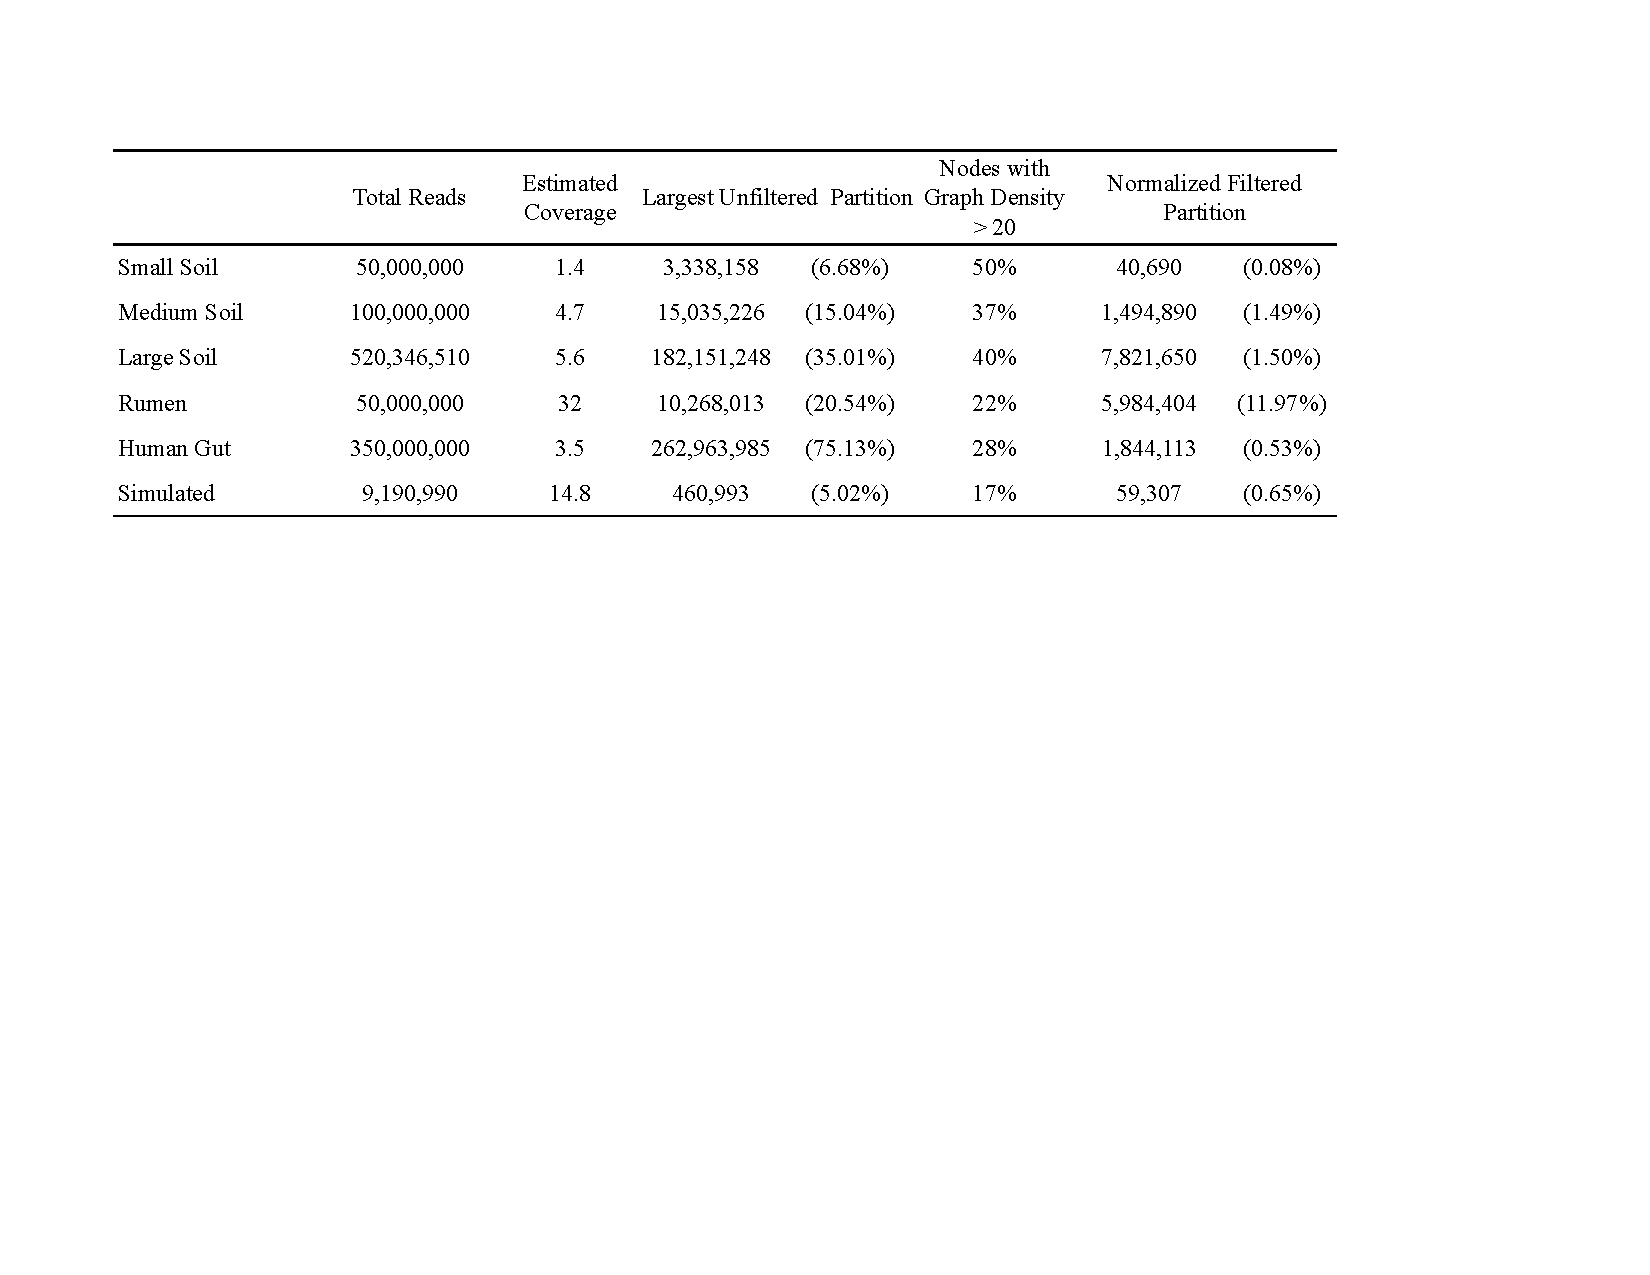
\includegraphics[width=5in]{./Figures/lump_data.pdf}}
\caption{The connectivity of sequencing reads from medium to high complexity metagenomes from the soil, rumen, and human-gut were analyzed.  Read coverage was estimated by aligning sequencing reads to Velvet-assembled contigs (K=33).  A dominant lump, or largest disconnected component of each metagenome assembly graph, was identified in each metagenome. }
\end{table}

\begin{figure}
\center{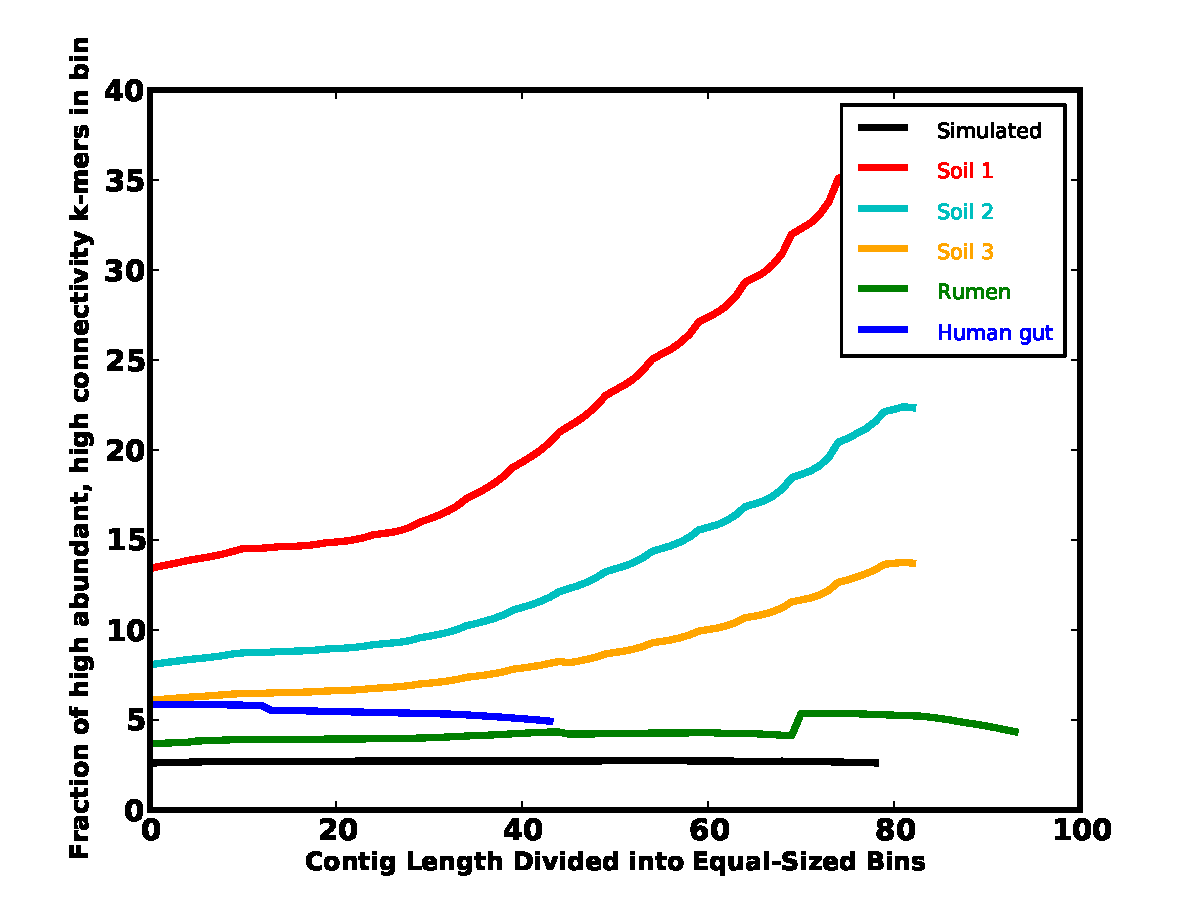
\includegraphics[width=5in]{./Figures/density_pos.pdf}}
\caption{The extent to which average local graph density varies by read position is shown for the lump of various datasets.  Unlike the graph density of the simulated metagenome lump, average graph density of sequences in metagenomic lumps varied significantly by position along the read.}
\end{figure}

\begin{figure}
\center{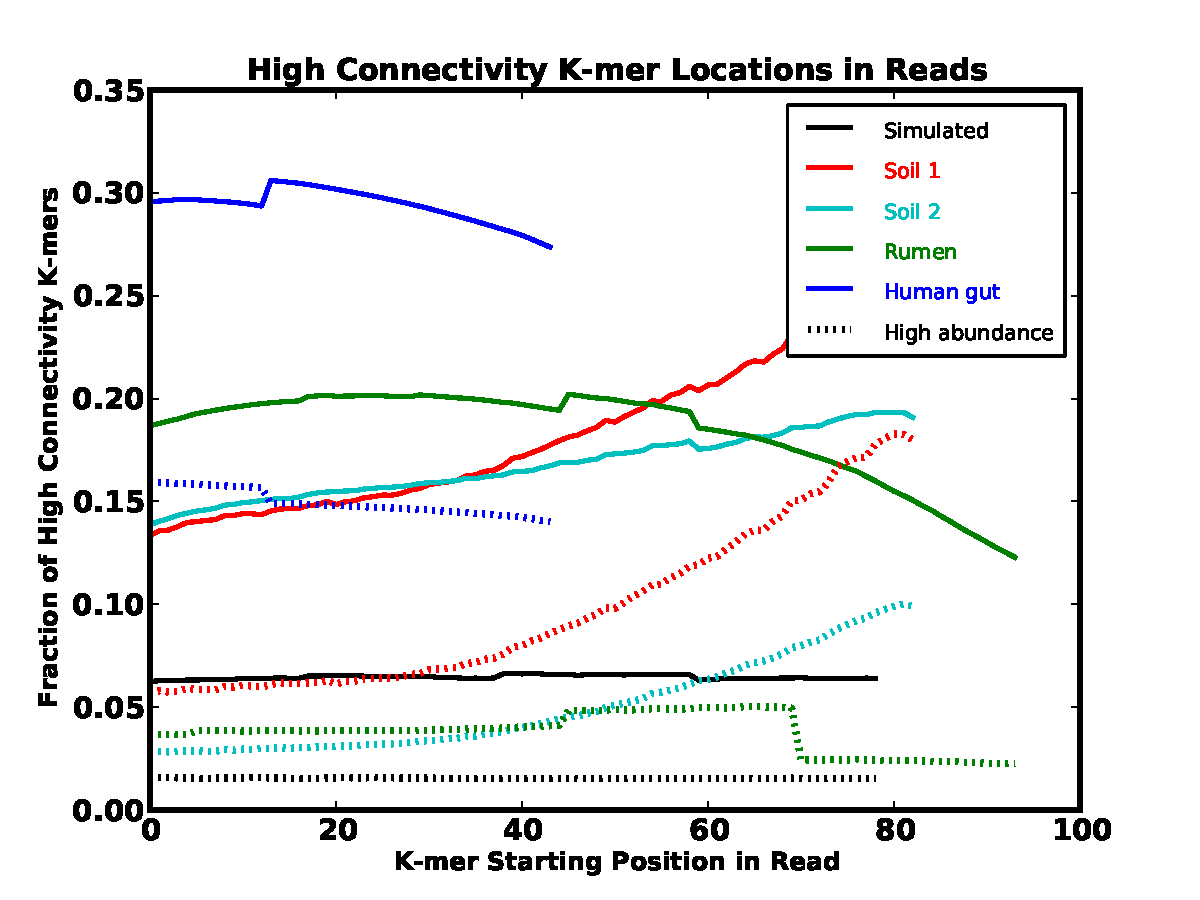
\includegraphics[width=5in]{./Figures/position_read_stoptags.pdf}}
\caption{The extent to which highly-connecting k-mers are present at specific positions within sequencing reads for various metagenomes.}
\end{figure}

\begin{table}
\center{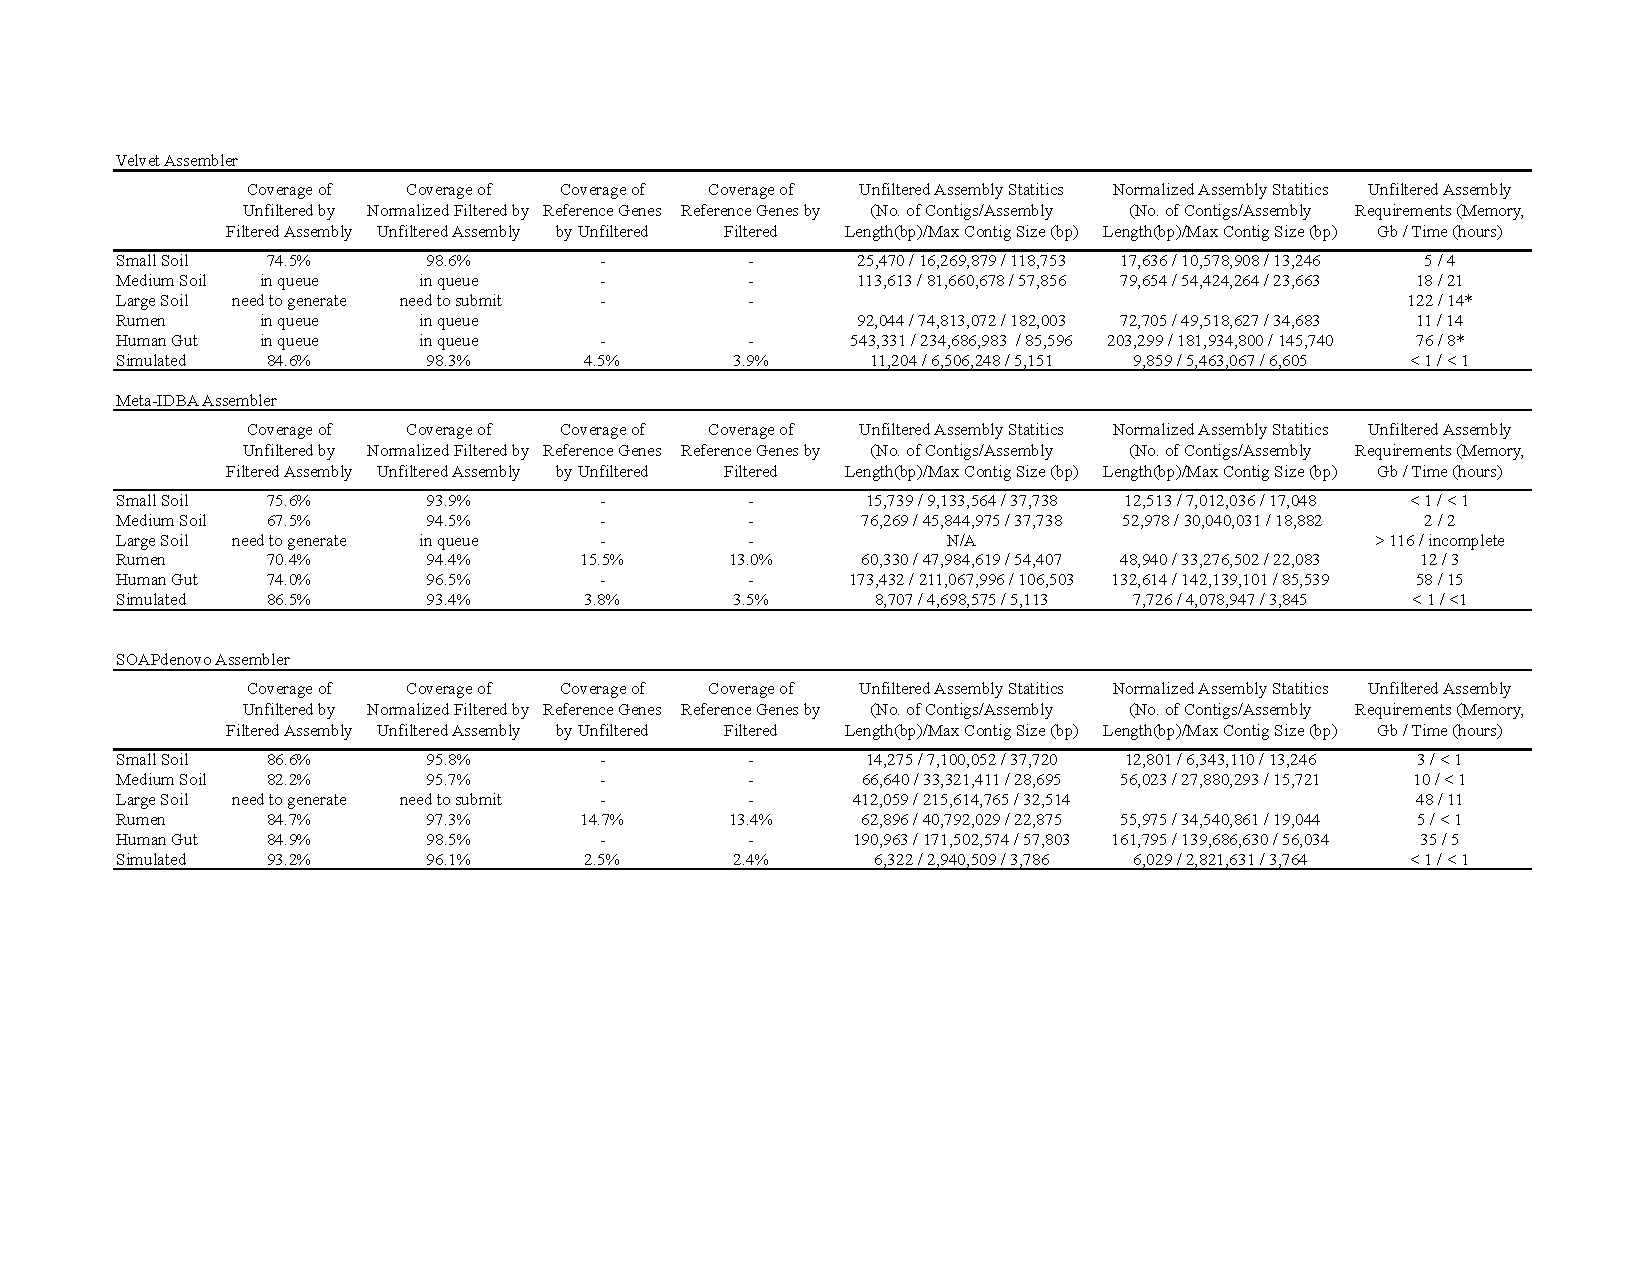
\includegraphics[width=5in]{./Figures/assembly_comparison.pdf}}
\caption{Comparison of unfiltered and filtered (removal of highly connecting k-mers) assemblies of various metagenome lumps.}
\end{table}

%\begin{figure}
%\center{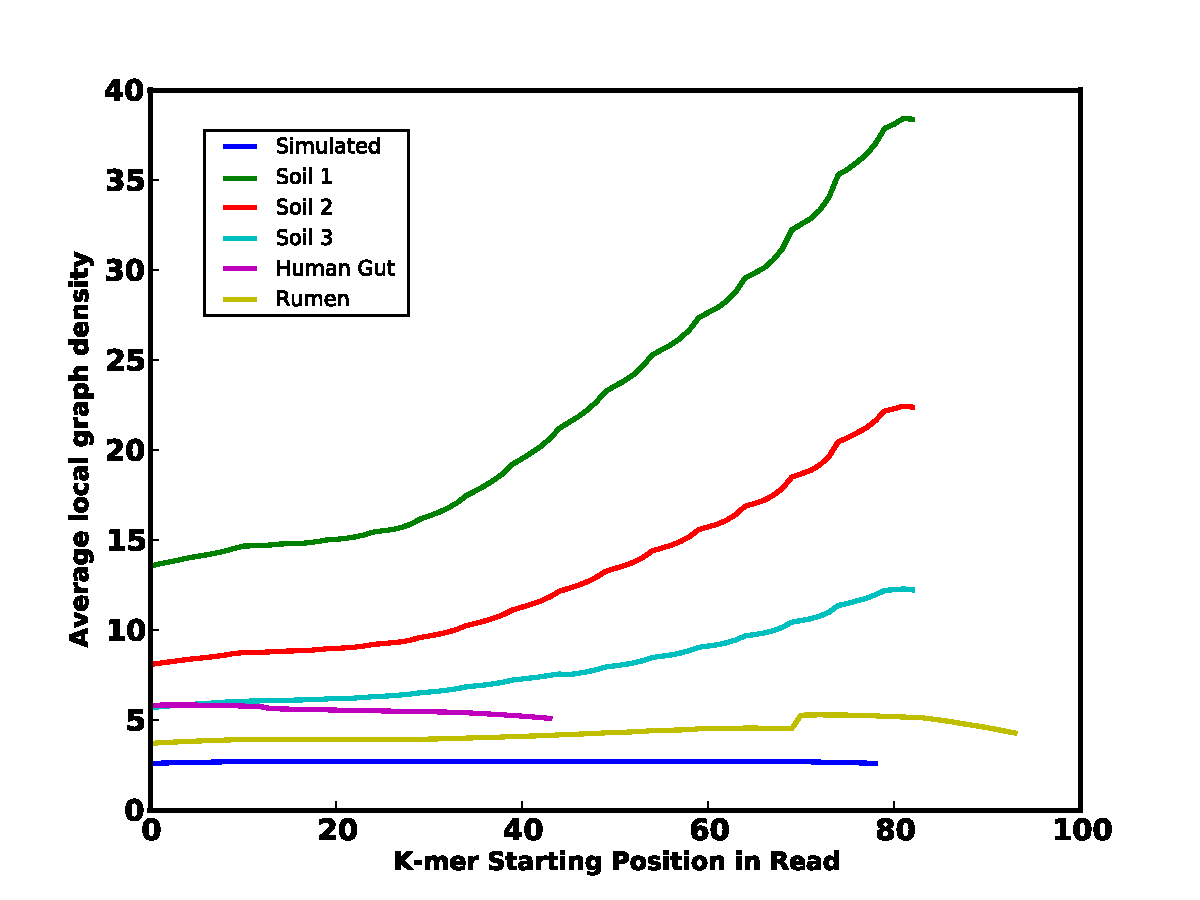
\includegraphics[width=5in]{./figures/density_pos.pdf}}
%\caption{Venn Diagram.}
%\end{figure}

\begin{figure}
\center{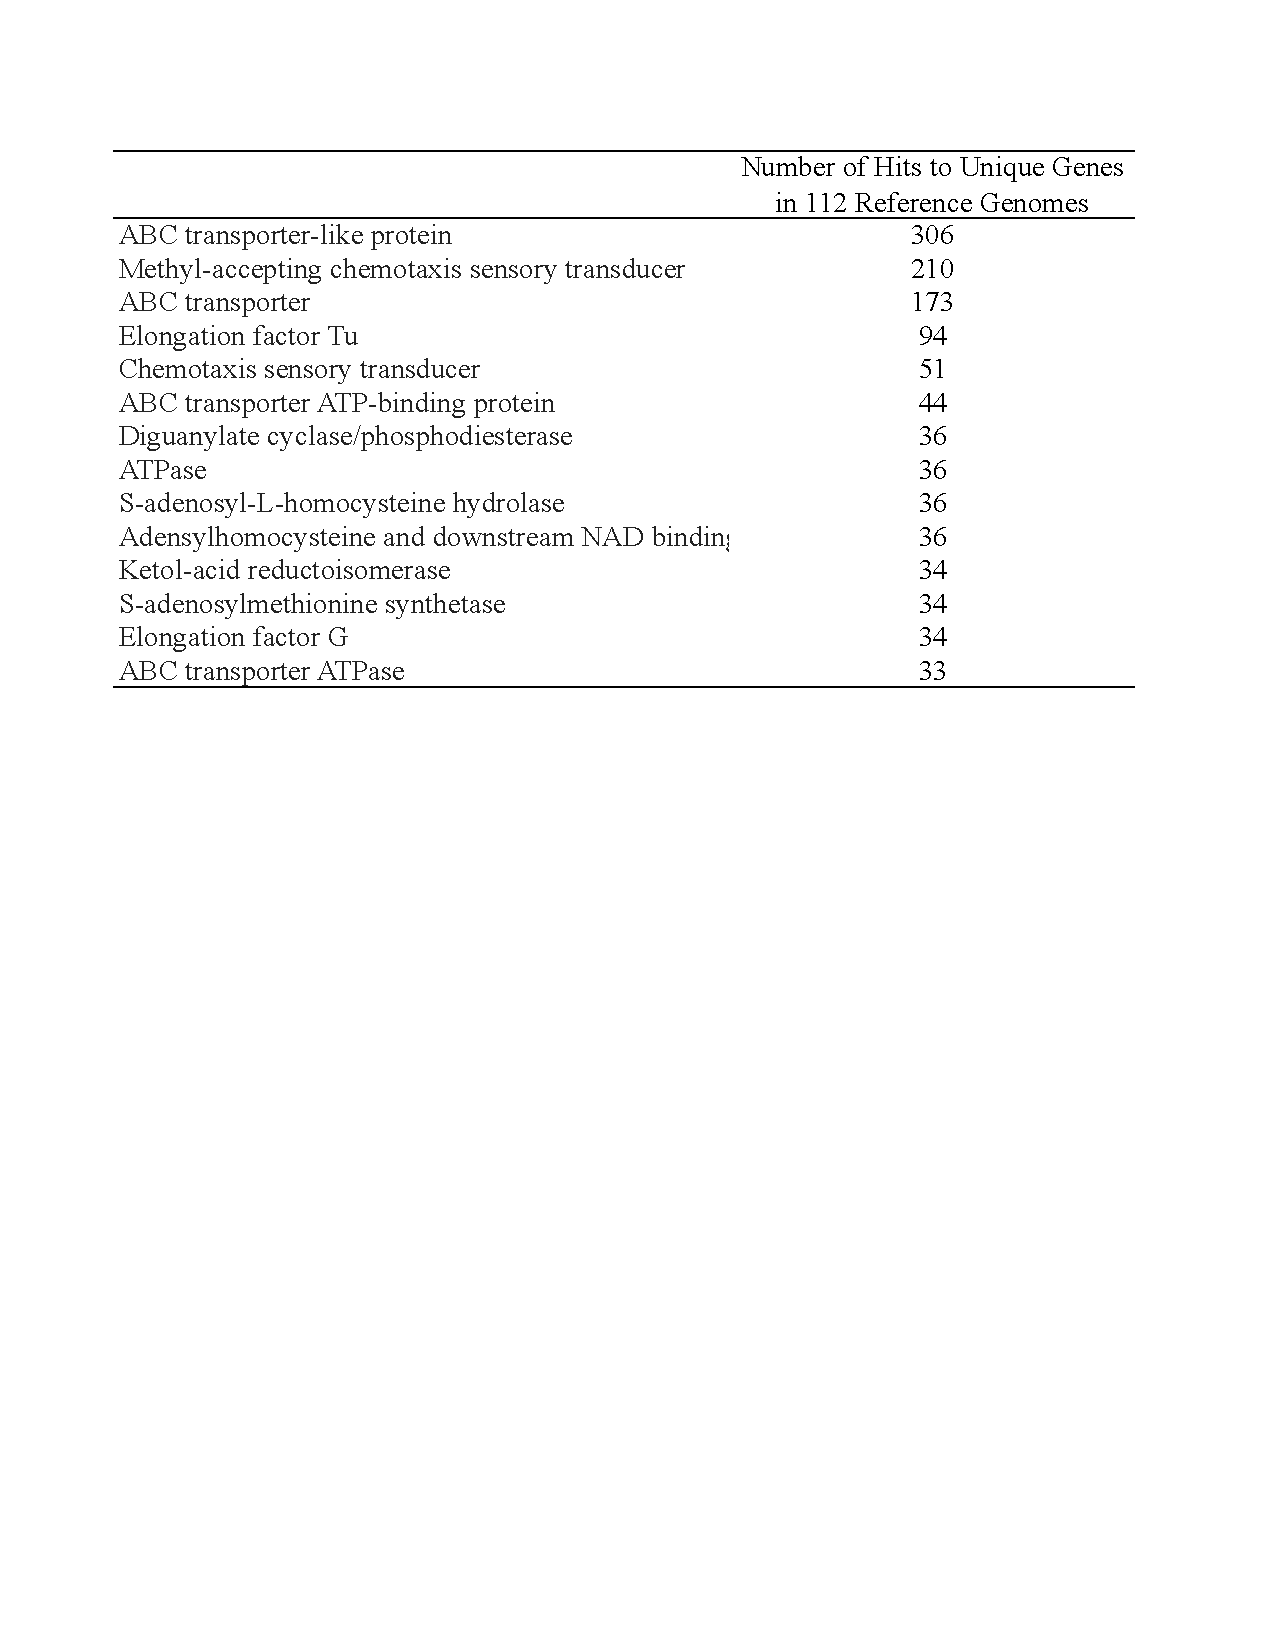
\includegraphics[width=5in]{./Figures/simulated_stoptag_ids.pdf}}
\caption{Annotation of highly-connecting sequences from the simulated metagenome with most hits to conserved genes within the 112 reference genomes (Pignatelli cite).  }
\end{figure}

\begin{figure}
\center{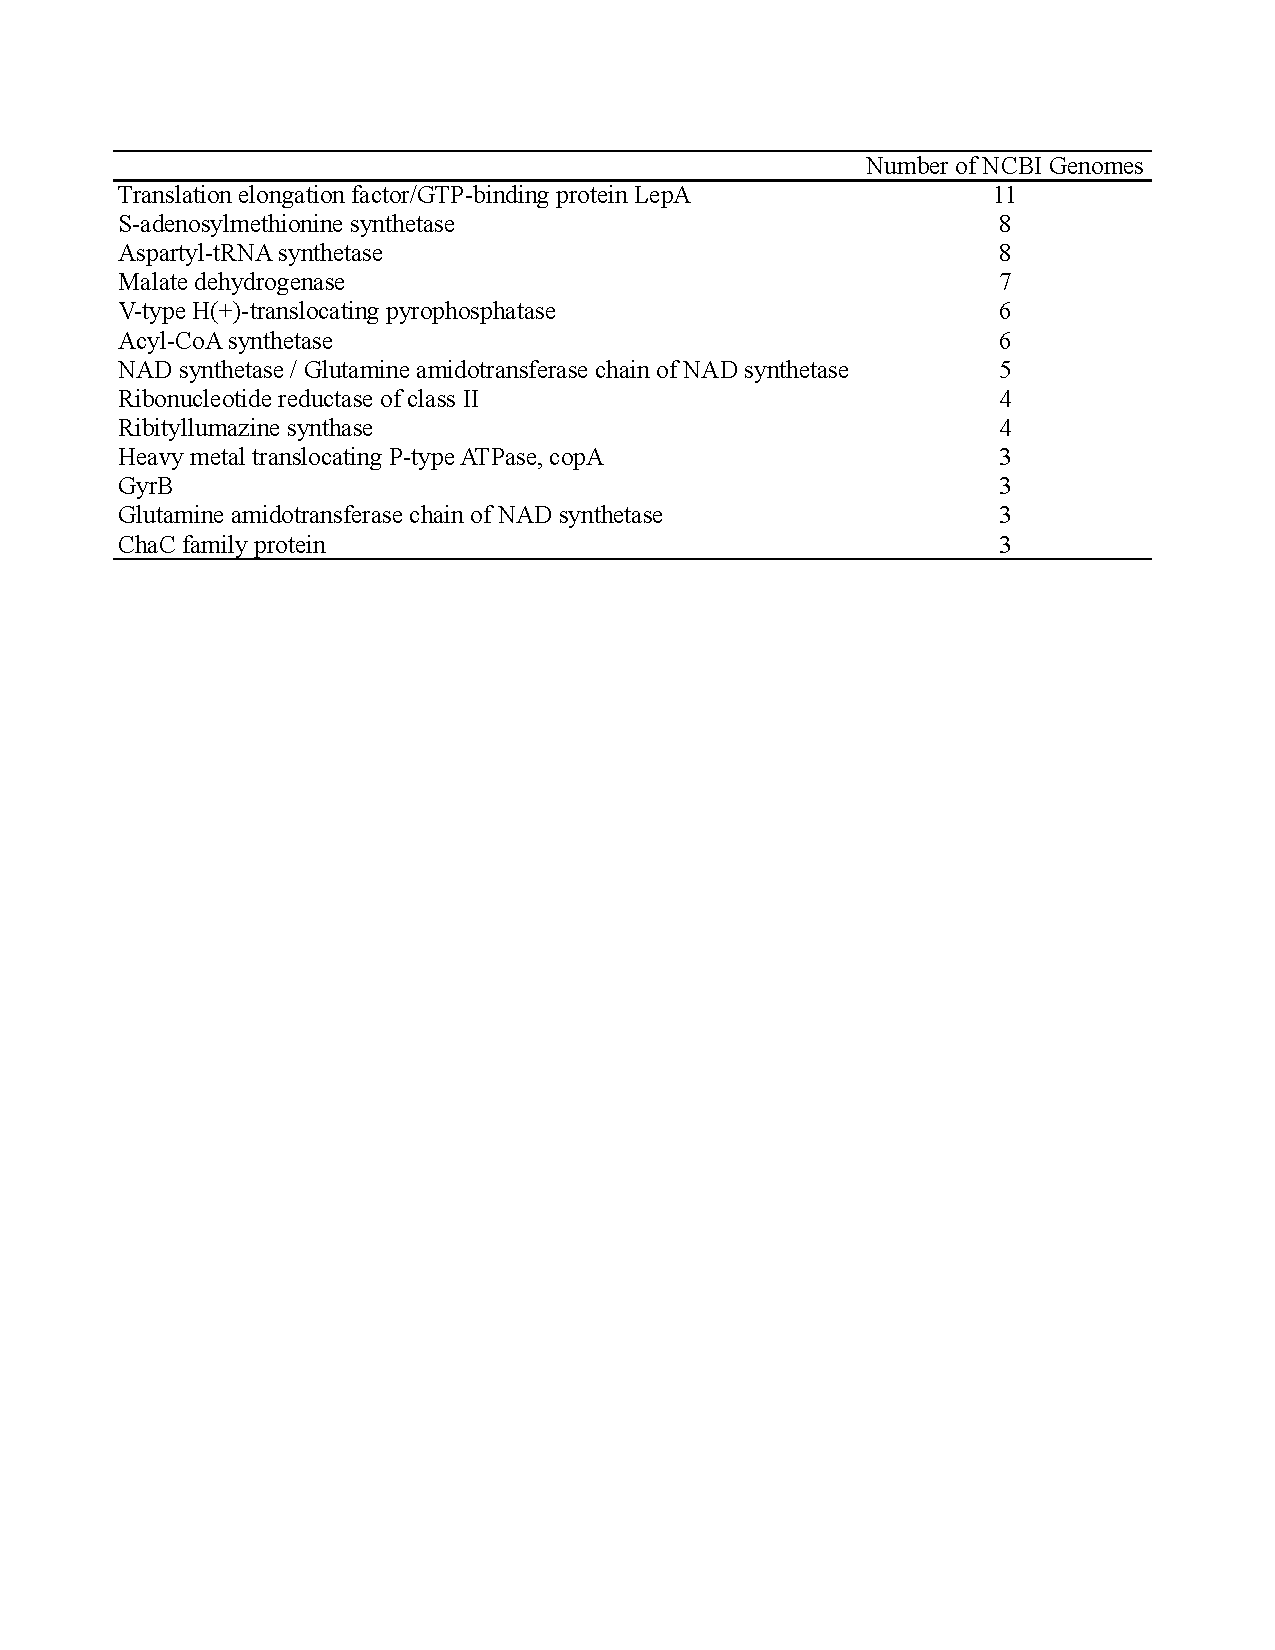
\includegraphics[width=5in]{./Figures/overlap_stoptag_ids.pdf}}
\caption{Annotation of highly-connecting sequences to conserved nucleotide sequences originating from 3 or more reference genomes.  Shown here are protein annotations whose nucleotide sequences matched 3 or more highly-connecting sequences shared in the three soil, rumen, and human gut metagenomes.}
\end{figure}



\begin{figure}
\center{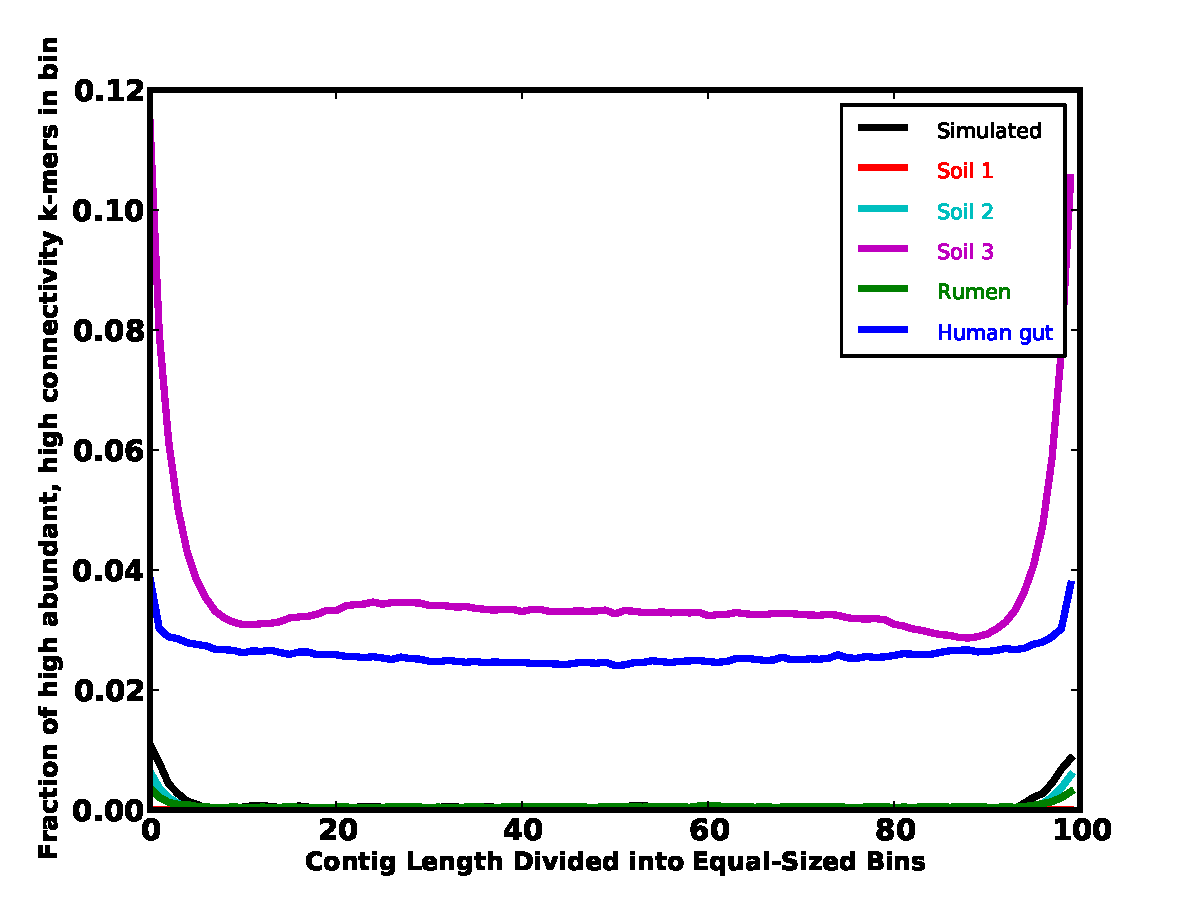
\includegraphics[width=5in]{./Figures/contig_pos_stoptags.pdf}}
\caption{When incorporated into an assembly, highly-connecting sequences (k-mers) were disproportionately present at the ends of contigs.}
\end{figure}

\section{Methods}

\subsection{Metagenomic datasets}
All datasets, with the exception of the agricultural soil metagenome, were from previously published datasets. Rumen-associated sequences (Illumina) were randomly selected from the rumen metagenome available at ftp://ftp.jgi-psf.org/pub/rnd2/Cow\_Rumen \cite{Hess:2011p686}. Human-gut associated sequences (Illumina) of samples MH0001 through MH0010 were obtained from ftp://public.genomics.org.cn/BGI/gutmeta/Raw\_Reads \cite{Qin:2010p189}. The agricultural soil metagenome was from an Iowa corn soil metagenome and is currently unpublished. All reads used in this study were quality-trimmed for Illumina's read segment quality control indicator, where a quality score of 2 indicates that all subsequent regions of the sequence should not be used. After quality-trimming, only reads with lengths greater than 30 bp were retained. All quality trimmed reads used in this study are available at X.  The number of reads after quality-trimming is shown in Table 1 for each metagenome. The simulated high complexity, high coverage dataset was previously published (Pignatelli, 2011).  

Coverage of each metagenome was estimated by aligning trimmed sequencing reads to assembled contigs with lengths greater than 500 bp.  For coverage estimates, the assembly of each metagenome was performed using Velvet (v1.1.05) with the following parameters:  K=33, exp cov=auto, cov cutoff=0, no scaffolding.  For datasets larger than 50 million reads, metagenomes were partitioned with the methods described in (cite PNAS paper) prior to assembly to overcome computational memory limitations for assembly.  Reads were aligned to assembled contigs with Bowtie (v0.12.7), allowing for a maximum of two mismatches.  

\subsection{Lightweight, compressible de Bruijn graph representation}
We used a lightweight probabilistic de Bruijn graph representation to explore k-mer connectivity of the assembly graph (cite PNAS paper). The de Bruijn graph stores k-mer nodes in Bloom filters and keeps edges between nodes implicitly, i.e. if two k-mer nodes exist with a k-1 overlap, then there is an edge between them. Bloom filters are a probabilistic set storage data structure with false positives but no false negatives, thus the size of the bloom filters were selected to be appropriate for each dataset and the memory available.
	
For analyzing the graph connectivity of the studied datasets, we used 4 x 48e9 bit bloom filters for soil, rumen, and human gut datasets, and 4 x 1e9 bit bloom filters for the simulated dataset. As metagenomic sequencing contains a mixture of multiple organisms, we could exploit the biological structure of the sequencing by partitioning the assembly graph into disconnected subgraphs that represent the original DNA sequence components. The set of the largest number of reads which were connected in the assembly graph is referred to above as a single, highly-connected lump. 

\subsection{Local graph density and identifying highly-connected k-mers}
We implemented a systematic traversal algorithm to identify highly connected components of the assembly graph.  Waypoints were labeled to cover the graph such that they are a minimum distance of L apart. Originating from a waypoint, all k-mers were systematically and exhaustively traversed within a region that is the distance N.   The local graph density was calculated as the number of X k-mers reachable within a distance N divided by the distance N.  Thus, the local graph density of a linear sequence would be 2, and additional branches or repeats would increase graph density.   To evaluate the extent of connectivity within each metagenomic lump, we calculated the number of nodes (K=32) with a local graph density greater than 20 when N=100 and determined these nodes to be "highly dense" (Table 2).  We also evaluated the degree to which graph density varied by position along a read.  For each k-mer in a read, the local graph density within N=10 nodes was calculated, and the total average local graph density by k-mer position for all reads was subsequently calculated (Figure 2).

\subsection{Characterization of effects of high abundance, high connectivity k-mers}

\subsubsection{Graph Traversal}
 
Highly connected k-mers were identified through exhaustive graph traversal using the bloom filter assembly graph representation.  We identified k-mers that were reachable from many locations in the graph.  Waypoints were labeled to cover the graph such that they
are a minimum distance of L apart.  Originating from a waypoint, all k-mers are systematically and exhaustively traversed within a region that is the distance L.  Such excursions that cover more than N k-mers are identified as "big excursions'', and k-mers that are present
in more than five big excursions are labelled as knots.  Local graph density (G) is defined as the number of k-mers within a specified region, or N/L.   For this study, L = 40 k-mer nodes, N = 200 k-mer nodes, and G > 5 is considered a big excursion.  

\subsubsection{Normalization}

To identify the high abundant k-mers which cause high connectivity, it was necessary to first minimize the effects of high coverage due to increased sequence sampling.  Using a digital normalization approach designed to remove redundant reads (cite paper), we assumed a maximum coverage per read (C=5) and thus minimized the affects of high coverage sequencing.  Subsequently, the set of k-mers which were identified as highly-connected with a coverage > 50 were considered highly abundant.  

\subsection{De Novo Metagenomic Assembly}

De novo metagenomic assembly of reads within each metagenomic lump was completed with Velvet (v1.1.02) with the following parameters: velveth -short -shortPaired (if applicable to the dataset) and velvetg -exp\_cov auto -cov\_cutoff 0 -scaffolding no \cite{Zerbino:2008p665}.  For the small and medium soil, rumen, and simulated metagenomes, assemblies were performed at K=25-49, dereplicated sequences with 99\% similarity with CD-HIT (v 4.5.6), and merged with Minimus (Amos v3.1.0, \cite{Sommer:2007p1253}).  For soil 3 and human gut metagenomes, assemblies were performed at only K=33 due to the size of the datasets and memory limitations.  

To compare unfiltered and filtered assemblies, we compared the total number of contigs, total assembly length, and maximum contig size.  Additional, the coverage of each assembly was calculated through estimating the average base pair coverage of the BLAST alignment of each assembly to one another.  

ORFs were predicted using Fraggenescan(v1.1.15) with the following parameters: -complete=0 -training=454\_10 \cite{Rho:2010p397}.   To identify biological sources of highly connective k-mers, sequences were aligned to original source genes and/or genomes through BLAST against specified databases.

The location of highly-connecting k-mers within assembled unfiltered contigs was examined by dividing each contig into 100 equally-sized regions.  The fraction of highly-connecting k-mers within each region was calculated for each metagenome.
 

\bibliography{artifacts-paper-bib}
\bibliographystyle{plain}


\end{document}







